\section{Application: Systems of linear differential equations}

In this section, we use some concepts from calculus. Recall that if
$y=f(x)$ is a function, then $y' = f'(x)$ is its derivative%
\index{derivative} and $y'' = f''(x)$ is its second derivative.  For
example,
\begin{equation*}
  \begin{array}{c@{~}c@{~}c}
    y &=& \sin(x),\\
    y' &=& \cos(x),\\
    y''&=& -\sin(x).\\
  \end{array}
\end{equation*}
Note that if $y=\sin(x)$, the function $y''$ is exactly the negative
of $y$, i.e.,
\begin{equation}
  y'' = -y.
\end{equation}
This last equation is called a \textbf{differential equation}%
\index{equation!differential|see{differential equation}}%
\index{differential equation}. Unlike an ordinary equation, which is
about an unknown {\em number}, a differential equation is about an
unknown {\em function}. Typically, a differential equation mentions
the function and one or more of its derivatives. A differential
equation that only mentions the first derivative $y'$ is called a
\textbf{first-order}%
\index{differential equation!first order} differential equation. A
differential equation that also mentions the second derivative $y''$
is called a \textbf{second-order}%
\index{differential equation!second order} differential equation.

We say that the function $y=\sin(x)$ is a \textbf{solution}%
\index{differential equation!solution} of the differential equation
$y'' = -y$. It is not the only solution. Another solution is
$y=\cos(x)$, because in that case, $y''=-\cos(x)$, and therefore
$y''=-y$. From calculus, we know the the \textbf{general solution} to
the differential equation $y'' = -y$ is given by
\begin{equation*}
  y = a\sin(x) + b\cos(x),
\end{equation*}
where $a$ and $b$ are any real numbers, i.e., parameters. Using the
terminology of linear algebra, we can say that the general solution to
the equation $y'' = -y$ is a {\em linear combination} of the basic
solutions $y=\sin(x)$ and $y=\cos(x)$. More generally, we have the
following theorem from calculus:

\begin{theorem}{Solutions of $y''=-ky$}{differential-equation}
  Let $k$ be a positive real number.  The general solution of the
  differential equation $y'' = -ky$ is
  \begin{equation*}
    y = a\sin(\sqrt{k}x) + b\cos(\sqrt{k}x).
  \end{equation*}
\end{theorem}

\begin{proof}
  We can check that it is a solution. By the chain rule, we have:
  \begin{equation*}
    \begin{array}{c@{~~}c@{~~}l}
      y &=& a\sin(\sqrt{k}x) + b\cos(\sqrt{k}x), \\
      y' &=& a\sqrt{k}\cos(\sqrt{k}x) - b\sqrt{k}\sin(\sqrt{k}x), \\
      y'' &=& -ak\sin(\sqrt{k}x) - bk\cos(\sqrt{k}x). \\
    \end{array}
  \end{equation*}
  Therefore $y''=-ky$. The fact that it is the most general solution
  is proved in a calculus course.
\end{proof}

One of the reasons that differential equations are important is that
the \textbf{laws of nature}%
\index{laws of nature} often take the form of differential equations.
For example, \textbf{Newton's second law of motion} asserts that the
vector sum of the forces $F$ on an object is equal to the mass $m$ of
the object multiplied by the acceleration $y''$ of the object, or in
formulas:
\begin{equation*}
  F = my''.
\end{equation*}
This is a differential equation. In physics, forces are caused by many
phenomena, but in the following examples, we will focus on forces
caused by \textbf{springs}%
\index{spring (mechanics)}. A spring is an object (often in the shape
of a coil) made from an elastic material, which returns to its
original shape after being stretched or compressed. The force exerted
by a spring follows \textbf{Hooke's law}%
\index{spring (mechanics)!Hooke's law}%
\index{Hooke's law}, which states that
\begin{equation*}
  F = -k x.
\end{equation*}
Here $x$ is the \textbf{extension}%
\index{spring (mechanics)!extension} of the spring, i.e., the change
in length of the spring, relative to its relaxed (natural)
length. Also, $k$ is a constant called the \textbf{spring constant}%
\index{spring (mechanics)!spring constant}.

\begin{example}{A mass and a spring}{mass-spring}
  Consider a train car of mass $1\kg$ on a track, connected to a
  stationary object by a spring with spring constant
  $k=1\frac{\SI{N}}{\m}$. Write down the equation of motion and then
  solve it.
  \begin{center}
    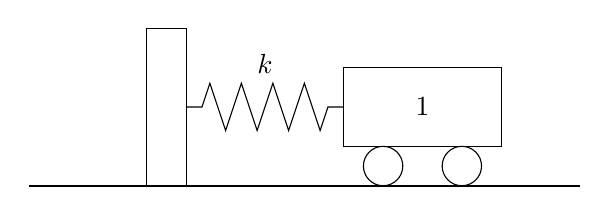
\begin{tikzpicture}
      \draw[fill=white] (-0.5,0) -- (-0.5,2) -- (0,2) -- (0,0);
      \draw[thick] (-2,0) -- (5,0);
      \draw[fill=white] (2,0.5) rectangle node {$1\kg$} (4,1.5);
      \draw[fill=white] (2.5,0.25) circle (0.25);
      \draw[fill=white] (3.5,0.25) circle (0.25);
      \draw (0,1) -- (0.2,1) -- ++(0.1,0.3)
      -- ++(0.2,-0.6) -- ++(0.2,0.6)
      -- ++(0.2,-0.6) -- ++(0.2,0.6)
      -- ++(0.2,-0.6) -- ++(0.2,0.6)
      -- ++(0.2,-0.6) -- ++(0.1,0.3)
      -- (2,1);
      \draw (1,1.3) node[above] {$k$};
    \end{tikzpicture}
  \end{center}
\end{example}

\begin{solution}
  Let us use the variables $t$ for time and $x$ for the horizontal
  displacement of the car, counted positively in the right direction.
  Let us further choose the coordinate system so that $x=0$
  corresponds to the position of the car when the spring is in its
  relaxed state.
\end{solution}

Consider the following mechanical system: three train cars of mass
$1\kg$, $2\kg$, and $1\kg$ are aligned on a track and connected by
springs. Each spring has the same spring constant
$k=1\frac{\SI{N}}{\m}$.
\begin{equation*}
  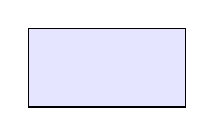
\begin{tikzpicture}
    \draw[fill=blue!10] (0,0) rectangle (2,1);
  \end{tikzpicture}
\end{equation*}



% ======================================================================
\subsection{CONTINUE HERE...}

  A
differential equation of the form $ay''+by'+cy = 0$ is called a
(homogeneous second order) \textbf{linear differential equation}%
\index{differential equation!linear}. Note
that the equation {\eqref{eqn:differential1}} is of this form, with
$a=1$, $b=0$, and $c=1$. In this section, we will use linear algebra,
and in particular diagonalization, to solve systems of homogeneous
linear differential equations.

This type of behavior along with complex eigenvalues is typical of the
deviations from an equilibrium point in the Lotka Volterra system of
differential equations which is a famous model for predator-prey
interactions. These differential equations are given by
\begin{eqnarray*}
  x^{\prime } &=&x(a-by) \\
  y^{\prime } &=&-y(c-dx)
\end{eqnarray*}
where $a,b,c,d$ are positive constants. For example, you might have
$X$ be the population of moose and $Y$ the population of wolves on an
island.

Note that these equations make logical sense. The top says that the
rate at which the moose population increases would be $aX$ if there
were no predators $Y$.  However, this is modified by multiplying
instead by $(a-bY) $ because if there are predators, these will
militate against the population of moose.  The more predators there
are, the more pronounced is this effect. As to the predator equation,
you can see that the equations predict that if there are many prey
around, then the rate of growth of the predators would seem to be
high. However, this is modified by the term $-cY$ because if there are
many predators, there would be competition for the available food
supply and this would tend to decrease $Y^{\prime }$.

The behavior near an equilibrium point, which is a point where the
right side of the differential equations equals zero, is of great
interest. In this case, the equilibrium point is
\begin{equation*}
  x=\frac{c}{d}, y=\frac{a}{b}.
\end{equation*}
Then one defines new variables according to the formula
\begin{equation*}
  x+\frac{c}{d}=x,\ y=y+\frac{a}{b}.
\end{equation*}
In terms of these new variables, the differential equations become
\begin{eqnarray*}
  x^{\prime } &=&\paren{x+\frac{c}{d}} \paren{a-b\paren{y+\frac{a}{b}
                  }} \\
  y^{\prime } &=&-\paren{y+\frac{a}{b}} \paren{c-d\paren{x+\frac{c}{d}
                  }}.
\end{eqnarray*}
Multiplying out the right sides yields
\begin{eqnarray*}
  x^{\prime } &=&-bxy-b\frac{c}{d}y, \\
  y^{\prime } &=&dxy+\frac{a}{b}dx.
\end{eqnarray*}
The interest is for $x,y$ small and so these equations are essentially
equal to
\begin{equation*}
  x^{\prime }=-b\frac{c}{d}y,\ y^{\prime }=\frac{a}{b}dx.
\end{equation*}
Replace $x^{\prime }$ with the difference quotient
$\frac{x(t+h) -x(t) }{h}$ where $h$ is a small positive number and
$y^{\prime } $ with a similar difference quotient. For example one
could have $h$ correspond to one day or even one hour. Thus, for $h$
small enough, the following would seem to be a good approximation to
the differential equations.
\begin{eqnarray*}
  x(t+h) &=&x(t) -hb\frac{c}{d}y, \\
  y(t+h) &=&y(t) +h\frac{a}{b}dx.
\end{eqnarray*}
Let $1,2,3,\ldots$ denote the ends of discrete intervals of time
having length $h$ chosen above. Then the above equations take the form
\begin{equation*}
  \begin{mymatrix}{c}
    x(n+1) \\
    y(n+1)
  \end{mymatrix} =\begin{mymatrix}{cc}
    1 & -\frac{hbc}{d} \\
    \frac{had}{b} & 1
  \end{mymatrix} \begin{mymatrix}{c}
    x(n) \\
    y(n).
  \end{mymatrix}
\end{equation*}
Note that the eigenvalues of this matrix are always complex.

We are not interested in time intervals of length $h$ for $h$ very
small.  Instead, we are interested in much longer lengths of
time. Thus, replacing the time interval with $mh$,
\begin{equation*}
  \begin{mymatrix}{c}
    x(n+m) \\
    y(n+m)
  \end{mymatrix} =\begin{mymatrix}{cc}
    1 & -\frac{hbc}{d} \\
    \frac{had}{b} & 1
  \end{mymatrix} ^{m}\begin{mymatrix}{c}
    x(n) \\
    y(n)
  \end{mymatrix}.
\end{equation*}
For example, if $m=2$, you would have
\begin{equation*}
  \begin{mymatrix}{c}
    x(n+2) \\
    y(n+2)
  \end{mymatrix} =\begin{mymatrix}{cc}
    1-ach^{2} & -2b\frac{c}{d}h \\
    2\frac{a}{b}dh & 1-ach^{2}
  \end{mymatrix} \begin{mymatrix}{c}
    x(n) \\
    y(n)
  \end{mymatrix}.
\end{equation*}
Note that most of the time, the eigenvalues of the new matrix will be
complex.

You can also notice that the upper right corner will be negative by
considering higher powers of the matrix. Thus letting $1,2,3,\ldots$
denote the ends of discrete intervals of time, the desired discrete
dynamical system is of the form
\begin{equation*}
  \begin{mymatrix}{c}
    x(n+1) \\
    y(n+1)
  \end{mymatrix} =\begin{mymatrix}{rr}
    a & -b \\
    c & d
  \end{mymatrix} \begin{mymatrix}{c}
    x(n) \\
    y(n)
  \end{mymatrix},
\end{equation*}
where $a,b,c,d$ are positive constants and the matrix will likely have
complex eigenvalues because it is a power of a matrix which has
complex eigenvalues.

You can see from the above discussion that if the eigenvalues of the
matrix used to define the dynamical system are less than 1 in absolute
value, then the origin is stable in the sense that as
$n\rightarrow \infty$, the solution converges to the origin. If either
eigenvalue is larger than 1 in absolute value, then the solutions to
the dynamical system will usually be unbounded, unless the initial
condition is chosen very carefully. The next example exhibits the case
where one eigenvalue is larger than 1 and the other is smaller than 1.

The following example demonstrates a familiar concept as a dynamical system.
